\documentclass[a4paper,11pt]{article}
\usepackage[plain]{fullpage} 
\usepackage{graphicx}  
\usepackage{wrapfig}
\usepackage{float}
\usepackage{array}
\usepackage[hidelinks]{hyperref}
\usepackage{color}
\definecolor{light-gray}{gray}{0.95}
\usepackage{listings}
\lstset{
basicstyle=\scriptsize, 
morecomment=[l]{/*},
backgroundcolor=\color{light-gray}, 
xleftmargin=.10in,
xrightmargin=.10in,
language=C
}

\renewcommand{\arraystretch}{1.25} %vertical cell padding

\title{\textbf{Report: Assignment 3}}
\author{Group 9: \O yvin Richardsen, Sandor Zeestraten, Stian Habbestad}
\date{{Norwegian University of Science and Technology \\
TDT4258 Energy Efficient Computer Design \\}
\today}

\begin{document}
\maketitle
\bigskip\bigskip\bigskip\bigskip\bigskip\bigskip\bigskip\bigskip\bigskip

\begin{abstract}
In this assignment the goal is to program a simple computer game in C on a Linux-variant which runs on an AVR STK1000 development board. To accomplish this one needs to understand and write Linux device drivers for I/O. We therefore wrote our own drivers for operating LEDs and switches on the development board. The game we chose to implement is a simple puzzle game called Sokoban which used these drivers.
\end{abstract}

\newpage
\tableofcontents
\newpage

\section{Introduction}
In this exercise we start out with running a Linux-variant on the STK1000 development board from the SD card. Our main tasks were writing device drivers and controllers for using already existing Linux drivers. On top of that we needed to write a game that used all the devices. We'll show how we developed the different parts and how they all work together.

\section{Description and methodology}
The first step was getting a Linux-variant to run on the board so we had something to develop on. This turned out to be a bit problematic. The supplied guide was somewhat unclear on the different steps. Luckily there was an image of a precompiled Linux that we could extract to the SD card. 

Once Linux was up and running we started out with a simple "Hello world" program to verify that things were working. We then looked at how to communicate with the frame buffer in Linux. In the beginning we thought maybe this file had to be a kernel module as well, but we soon understood that we needed access to quite a few libraries to make the memory mapping work. We started with generating a random bit values for the display and went on with more logical values, for example a third of the screen was made red. We organized the screen into a grid of 20 by 15 tiles built up of 16 by 16 pixels for each tile. This made it easy to map the \textit{charmap} to the images and render the levels on the LCD screen. More on this in section~\ref{sec:lcd}.

After getting the framebuffer to work, we wrote the drivers and controllers for the LEDs and buttons. This took a while to perfect as we had to share one of the GPIO ports and manage to control the different pins separately. In the previous assignment we learned how to handle and generate sounds in C. However, for this assignment we decided to opt for reading in regular sound files instead. This saved us some time and avoided the complexity of composing and generating new sounds.

Once we managed to control all the device drivers we implemented the game. This was relatively simple as we had already written it in Java in a previous course. We'll now look at an overview of the main code for the game and introduce the different parts in more detail.

\subsection{Overview}
The game code can be split up into two main parts. The game engine and logic itself, and all the controllers that interface with the drivers. See section~\ref{sec:driversandcontrollers} for a more detailed explanation of the latter part. The main entry point of the game is in \textit{sokoban\_graphics.c}. It opens all the drivers via the controllers and loads the necessary media for the game. It then starts the game loop which can be seen in figure~\ref{fig:programflow}. 

\begin{figure}[H]
\centering
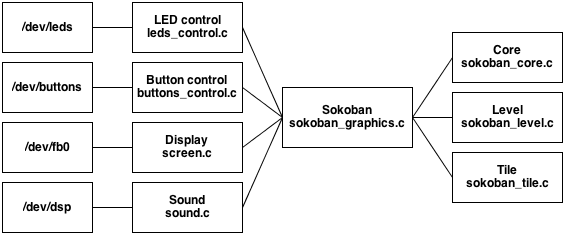
\includegraphics[scale=0.6]{images/blockdiagram.png}
\caption{A block diagram overview of the complete game.}
\label{fig:blockdiagram}
\end{figure}

\begin{figure}[H]
\centering
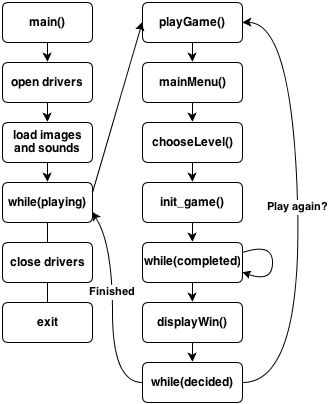
\includegraphics[scale=0.6]{images/programflow.png}
\caption{An overview of the main game flow in \textit{sokoban\_graphics.c}.}
\label{fig:programflow}
\end{figure}

\subsection{The game}
\subsubsection{Sokoban}
The game we chose to implement was a simple top-down puzzle game called \textit{Sokoban}\cite{sokoban}. The point of the game is for the player to push boxes onto marked target squares. The levels are small maps confined by walls which cannot be walked through. The puzzle is solved when all the boxes are on the target squares. We had some previous experience of implementing this game in Java in the course TDT4100: Object Oriented Programming. We therefore chose to port it to C. See figure~\ref{fig:sokobanscreen} for a screenshot of a level in Sokoban.

\begin{figure}[H]
\centering
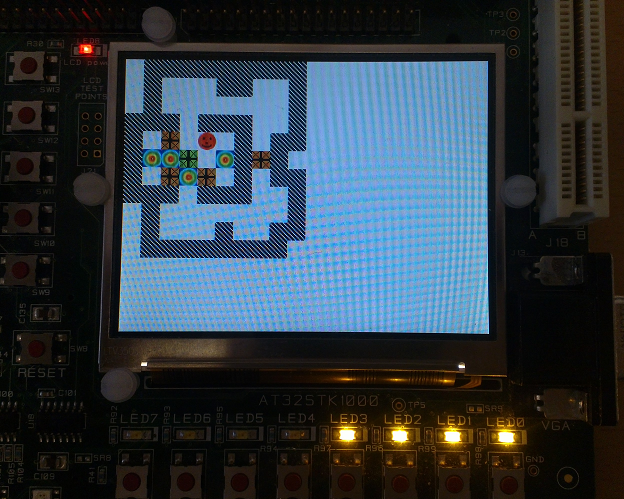
\includegraphics[scale=0.4]{images/sokobanscreen.png}
\caption{A screenshot of a level in Sokoban.}
\label{fig:sokobanscreen}
\end{figure}

\subsubsection{Levels}
The levels are defined by it's dimensions and an array of characters of the different elements. For more information see the level format page on Sokoban Wiki \cite{sokobanlevel}. The  table~\ref{tab:levelformat} shows the level format we used. For an example of how the levels are designed, see figure~\ref{fig:leveldef}. This is level 1 and it is the simplest solvable level. The only move available is to push the box to the right. Figure~\ref{fig:level1} shows how it looks on the STK1000.

\begin{table}[H]
\centering
\begin{tabular}{|l|l|l|}
\hline \textbf{Level element} & \textbf{Character} & \textbf{Graphics} \\ 
\hline Wall & \# & 
\includegraphics[scale=0.6]{images/wall.png} \\ 
\hline Player & @ & 
\includegraphics[scale=0.6]{images/player.png} \\ 
\hline Player on target square & + & 
\includegraphics[scale=0.6]{images/playertarget.png} \\ 
\hline Box & \$ & 
\includegraphics[scale=0.6]{images/crate.png}\\ 
\hline Box on target square & * & 
\includegraphics[scale=0.6]{images/cratetarget.png}\\ 
\hline Target square & . & 
\includegraphics[scale=0.6]{images/target.png}\\ 
\hline Floor & (whitespace) & 
\includegraphics[scale=0.6]{images/blank.png} \\ 
\hline 
\end{tabular}
\caption{The level format.}
\label{tab:levelformat}
\end{table}

\begin{figure}[H]
\begin{lstlisting}
// From sokoban_leveldefs.h
#define level1dimX 5
#define level1dimY 3
char level1[] = "######@$.######";
\end{lstlisting}
\caption{Definition of the level 1.}
\label{fig:leveldef}
\end{figure}

\begin{figure}[H]
\centering
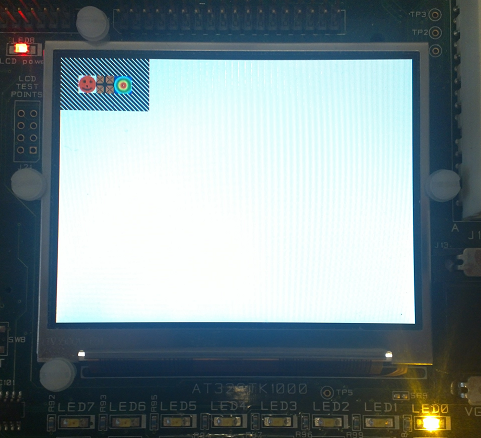
\includegraphics[scale=0.5]{images/level1.png}
\caption{Level 1 running on the STK1000.}
\label{fig:level1}
\end{figure}

\subsubsection{Game logic}
The game logic itself is reasonably simple. One needs to load a level, identify the different characters, draw the level, then check if the player move is valid. The more tricky part is allowing for undo/redo where one has to keep track of the history of all the moves the player makes. The files \textit{sokoban\_core.c}, \textit{sokoban\_level.c} and \textit{sokoban\_tile.c} handle most of the game logic.

\subsection{Drivers and controllers}
\label{sec:driversandcontrollers}
In order to interact with the development board we wrote two separate device drivers. One for the LEDs and one for the buttons. In addition we used the framebuffer device to display images on the LCD and for sound we used the built in sound driver in Linux.

\begin{figure}[H]
\centering
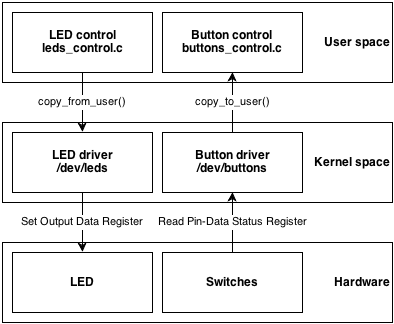
\includegraphics[scale=0.6]{images/devicedrivers.png}
\caption{An overview of the device drivers we wrote in the kernel and user space.}
\label{fig:devicedrivers}
\end{figure}

\subsubsection{LEDs}
For the LEDs, we had to write both a driver for the actual I/O to the pins, and a controller to interface with the LED driver device.
\paragraph{Driver} The LED driver (\textit{leds.c}) is rather simple; By following the examples in chapter 3 and 9 of the Linux Device Drivers guide\cite{ldd}, we allocated minor and major numbers for the (char) device, requested access to the necessary I/O pins (pins 8-30 on PIO B), initialized these for LED use, and registered the device and its file operations in the system. For our purpose, we only had to implement functionality in the \textit{write()} file operation, as we only need to set the value of these I/O ports. We used a support function, \textit{set\_leds()}, to write the correct data to the correct ports based on input from the controller. We also implemented support for releasing major/minor numbers and reserved ports when deactivating the driver.
\paragraph{Controller} The LED device controller (\textit{leds\_control.c}) is the interface module we use between the game logic and the LED driver. This module contains functions for opening and closing the LED driver device file, as well as functions for manipulating the LEDs in various ways as needed by our game. The controller writes one byte, indicating which of the 8 LEDs should be active, to the device file. Our only needs for the game is to blink all the LEDs when the game completes (performed by the function \textit{blink\_leds()}), and show as many LEDs as there are empty targets on the board (up to a maximum of 8, performed by the \textit{increment\_leds()} and \textit{decrement\_leds()} functions).

\subsubsection{Buttons}
For the buttons, we also had to write both a driver for the I/O ports and a controller to interface with this driver.
\paragraph{Driver} For the button driver, \textit{buttons.c}, we followed mostly the same procedure as with the LED driver, except this time we implemented only the \textit{read()} file operation, in order to read the current status of the pins the buttons are connected to.
\paragraph{Controller} The button device controller (\textit{buttons\_control.c}) is very simple, and only holds functions for opening and closing the device file, reading the status of the buttons, and debouncing to avoid one button push activating a series of events.


\subsubsection{LCD} 
\label{sec:lcd}
For the LCD display, we only had to write a device controller, \textit{screen.c}, since a driver device (\textit{/dev/fb0}) for this already was active in the operating system. 
\paragraph{Controller} Like with the LEDs and buttons, the basic functions for opening and closing the device file had to be implemented in this controller (\textit{screen.c}). Additionally, we mapped the device file to memory, for simplified access to different parts of the file (we don't want to lseek every time we want access to a specific part of the file). We chose to use \textit{.bmp} files for the game graphics, so we implemented a function (\textit{read\_image\_data()}) for reading \textit{.bmp} pixel data into a memory array. Each pixel consists of 3 byte values, representing color values for blue, green and red. This representation is identical to the pixel format of the LCD display, so writing this data to the display driver proved to be rather straightforward (see \textit{write\_to\_screen()}), the only challenge being reversed order of pixel rows. We also implemented some support functions for the game. \textit{clear\_screen()} writes only white pixels to the whole display, \textit{display\_tile()} displays a square image with the given pixel dimension to the given tile position (which is then converted to pixel position), and \textit{display\_image()} displays a given fullscreen image.

\subsubsection{Sound}
Making the sound work properly, was probably the greatest challenge of the whole exercise. Fortunately, the sound driver was already in place (\textit{/dev/dsp}), so we only had to write the controller interfacing with this device. 
\paragraph{Controller} This controller (\textit{sound.c}) also implements functions to open and close the device file, but we also set the sample size (8 bits), number of channels (1) and sample rate of the device (8 kHz), to make sure these values are consistent with our own sound data. As with the graphics, we load our data from files (with \textit{load\_sound\_from\_file()}), and the format we use for sound files is unsigned 8 bit PCM encoded .wav.

For basic sound function, the easiest implementation would be to simply write sample data to the device on the fly, however this would be inconvenient, because it blocks any other functions until the sound has finished playing, and thus makes playing longer sounds a problem (playing music while playing the game would not be possible). We wanted to be able to continuously play music in addition to shorter sounds based on interaction in the game, while still maintaining a smooth input response. The first step towards this, was forking the write loop to a separate process, so that the program could continuously write samples to the device file without blocking other actions.

However, a new process gets its own variables and address space, so in order to control the sound from the main process, we had to map a shared memory file between the processes (see \textit{map\_shared\_memory()} and \textit{map\_pointers()}). The new process will simply run a loop (see \textit{loop\_sound()}) that reads samples from the shared memory, and writes these to the device file. The main process may then continue executing the game logic, and activate or deactivate sounds (\textit{play\_sound()} and \textit{stop\_sound()}) by writing sample data to the shared memory. This way, playing a new sound does not block the main process until the sound has played, which allows for smooth input response. Some additional data must be shared between the processes to make this work, like the length (in number of samples) of the current longest active sound (generally the music) and the position new samples should be written to in the shared memory.

\subsection{Debugging}
During the development of the drivers we often ran into various issues. As we now had a terminal we opted to make sure to print out the program state often in order to track down bugs. We also took care to check and exit the program when we were reading image and sound files. Figure~\ref{fig:consolestart} shows the terminal output of a successful load of the drivers and a run through of level 1 of the game.

\begin{figure}[H]
\centering
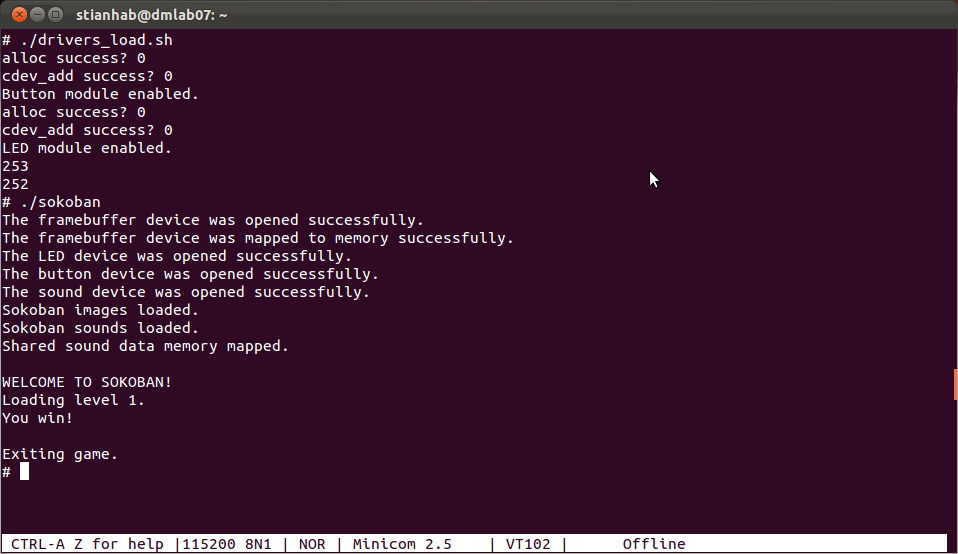
\includegraphics[scale=0.4]{images/consolestart.png}
\caption{Loading of device drivers and running the game from the console.}
\label{fig:consolestart}
\end{figure}

\section{How to setup, build and play}
\subsection{STK1000 setup}
Make sure that all the jumpers and cables are connected as described in section 4.3.3 in the TDT4258 Compendium \cite{komp}.
In addition, use the following setup for the GPIO, buttons and LEDs.

\begin{itemize}
\item Connect J1 to Switches
\item Connect J2 to Buttons
\end{itemize}

\subsection{Build instructions}
We've setup our build environment to automatically upload the necessary files to the development board. Should you want to upload and run the compiled binaries yourself, then simply upload the files found into the \textit{bin} directory to the \textit{root} directory of the board and continue with the run instruction.

\paragraph{Drivers}
In the \textit{driver} directory, edit the \textit{compile\_and\_upload\_drivers.sh} script and set the correct IP address of the board. Then run the script which compiles and uploads them.

\paragraph{Game}
In the \textit{sokoban} directory, edit the \textit{Makefile} and again edit the IP of the board. Then run \textit{make} and \textit{make send}.

\subsection{Run instructions}
Connect to the board with \textit{Minicom} as described in the compendium. Run the \textit{drivers\_load.sh} script to load the drivers. Then to start the game, simply run the \textit{sokoban} executable. See figure~\ref{fig:consolestart} for the console output if the drivers and the game run successfully. 

\section{Results}
\subsection{Game} 
This exercise resulted in a working Sokoban game on the STK1000 development board. The game is played by using the buttons as a controller to move around in the game which is displayed on the LCD screen. In addition to a general "arrow key" setup, there is also a possibility to undo and redo with the buttons. For a quick view of how the game operates see our gameplay video on Youtube\cite{youtube}. At the start of the program you are prompted with a main menu where you can choose between 8 different levels. After finishing a level you have the option to go back to the main menu or press \textit{SW7} to end the game.

\subsection{LEDs and sounds}
We've used the LEDs to show how many boxes there are left that need to be moved. If you complete a level the lights will also blink and display a splash screen. As for sounds, we have intro music in the main menu, background music while playing and song for when you win. These all continue looping. Also, while playing there are sound effects for when you move, push boxes on targets, and hit a wall.

\subsection{Game controls}
The setup of the buttons are not ideal for playing the game, but for those who are familiar with the Unix layout for arrow keys first used in Vi text editor, it will be easy to play. The controls of the game are listed below in table~\ref{tab:gamecontrols}. 

\begin{table}[H]
\centering
\begin{tabular}{|l|l|}
\hline \textbf{Switch} & \textbf{Action} \\ 
\hline SW7 & Move left \\ 
\hline SW6 & Move down \\ 
\hline SW5 & Move up \\ 
\hline SW4 & Move right \\ 
\hline SW3 & Undo move \\ 
\hline SW2 & Redo move \\ 
\hline SW1 & Reset level \\ 
\hline SW0 (x2) & Main menu \\
\hline 
\end{tabular}
\caption{Game controls} 
\label{tab:gamecontrols}
\end{table}

\section{Tests}
\subsection{Description}
We've created a few test scenarios in order to test different aspects of our game functionality. The tests were conducted by a person interacting with the switches and looking at the LCD screen, wearing a headset. Another person logged the results of the test. The main equipment was the STK1000 development board and a headset with the main focus on the LCD screen. The jumpers of the board were set as specified in the compendium (section 4.2) \cite{komp}. The GPIO was set up with both LEDs and switches connected to B as follows: LEDs on 8-15, switches on 0-7. 

\subsection{Results}
Below is a table of the different tests we ran, the preconditions and the results. 

\begin{center}
\scriptsize
\renewcommand{\arraystretch}{1.25} %vertical cell padding
\begin{tabular}[pos]{|m{35pt}|m{45pt}|m{80pt}|m{90pt}|m{105pt}|m{40pt}|}
\hline \textbf{Number} & \textbf{Name} & \textbf{Description} & \textbf{Conditions} & \textbf{Expected} & \textbf{Results} \\ 

\hline 1 & Steady-state test & Power is on and the main program is running & The board has been programmed and powered on & The board is powered and no LEDs or sounds should be on & Passed \\

\hline 2 & Left & Player is moved left & A level is loaded and there is free space to the left of the player & Player moves to the left when \emph{SW7} is pressed.  & Passed \\

\hline 3 & Down & Player is moved down & A level is loaded and there is free space beneath the player & Player moves down when \emph{SW6} is pressed.  & Passed \\

\hline 4 & Up & Player is moved up & A level is loaded and there is free space above the player & Player moves up when \emph{SW5} is pressed.  & Passed \\

\hline 5 & Right & Player is moved right & A level is loaded and there is free space to the right of the player & Player moves to the right when \emph{SW4} is pressed.  & Passed \\

\hline 6 & Undo & The last move is undone & At least one move is made & The last move is undone when \emph{SW3} is pressed.  & Passed \\

\hline 7 & Redo & The last undo is undone & Undo must have been done as the previous move. & The undone move is redone when \emph{SW2} is pressed.  & Passed \\

\hline 8 &  Reset level & The loaded level is reset & A level must have been loaded and the game may or may not have been initialized & Level is reset when \emph{SW1} is pressed.  & Passed \\

\hline 9 & Return to main menu & Main menu is displayed & Sokoban has been loaded. & Main menu is displayed when \emph{SW0} is pressed.  & Passed \\

\hline 10 & Return to main menu & Main menu is displayed & Sokoban is loaded and a game has been won. & Main menu is displayed when \emph{SW0} is pressed.  & Passed \\

\hline 11 & Undo after reset & Nothing happens & A sokoban level is loaded and the game may or may not have been initialized. & Nothing is supposed to happen.  & Passed \\

\hline 12 & Redo after reset & Nothing happens & A sokoban level is loaded and the game may or may not have been initialized. & Nothing is supposed to happen.  & Passed \\

\hline 
\end{tabular} 
\end{center}

\newpage

\section{Evaluation of assignment}
We found it interesting to learn more about the inner workings of Linux and how a device driver is written. We spent quite some time getting Linux to run on the STK1000 development board. This was much due to the original guide on the course site and Itslearning didn't really seem to work. At least no one that we talked to made it work by following that guide. After working together with another group who wrote the other guide posted later on Itslearning, we finally got it to work. 

\section{Conclusion}
During this exercise we have learned how to write Linux device drivers, how to run a Linux-variant on the STK1000 development board and implement a game in C on top of it. Most of the time was spent writing the drivers for controlling the LEDs and getting input from the buttons and also trying to interface with the other devices for the LCD and sound. 

\footnotesize{  % This makes the Reference items print in footnotesize fonts
\begin{thebibliography}{N}
\bibitem{ldd} Linux Device Drivers, Third Edition. Retrieved 04.04.13.
\url{http://http://lwn.net/Kernel/LDD3/}

\bibitem{sokoban} Description of the game Sokoban on Sokoban Wiki. Retrieved 23.04.13.
\url{http://www.sokobano.de/wiki/index.php?title=The_rules_of_the_game}

\bibitem{sokobanlevel} Description of Sokobon levels on Sokoban Wiki. Retrieved 23.04.13.
\url{http://www.sokobano.de/wiki/index.php?title=Level_format}

\bibitem{avrdoc} AVR32 Architecture Document.
\url{http://www.atmel.com/images/doc32000.pdf}

\bibitem{stkdoc} AT32AP7000 Datasheet.
\url{http://www.atmel.com/Images/doc32003.pdf}

\bibitem{komp} TDT4258 Compendium.
\url{http://www.idi.ntnu.no/emner/tdt4258/_media/kompendium.pdf}

\bibitem{youtube} Video of the Sokoban gameplay on Youtube. \url{https://www.youtube.com/watch?v=E7rSl4hEsEI}

\end{thebibliography}  
}
\end{document} 
